
\subparagraph{Register File Details : }
This section gives some expanded information on the operation
of the architected ISA register files.
Figure~\ref{registers2} shows a more detailed view
of two registers files each holding just two registers.

\begin{figure}
\centering
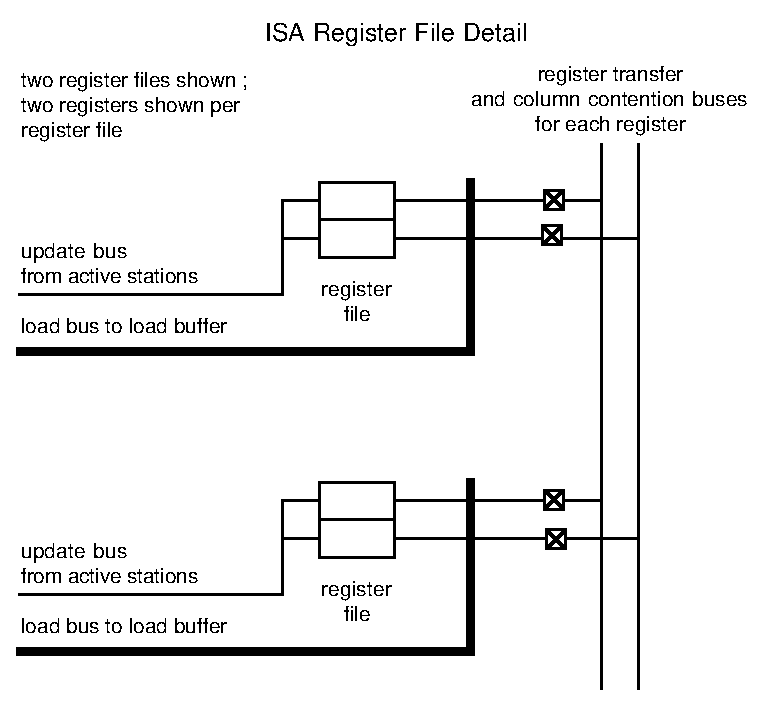
\epsfig{file=registers2.eps,height=1.50in}
\caption{{\em Timing of the code example, predication scenario 1.}
This example illustrates the exploitation of basic minimal control
dependencies, a significant contribution to
achieving higher ILP by taking advantage of independent
instructions beyond the joins of branches.
Execution of an instruction at a given time is
again indicated by an `X'.}
\label{registers2}
\end{figure}

The ISA register files serve the purpose
of maintaining the latest, or nearly the latest, versions of
all architected registers.  There is one register file
implemented per row of active stations in the instruction window.
Each register file contains a complete complement of all of
the ISA registers.

As instructions are fetched, they are staged for loading into the
instruction window using the load buffer.  Nominally, when the
instruction load buffer is full and the last (left-most) column of the
instruction window is ready to be retired, a shift-left load
operation occurs.  All register sources for the loaded instructions
must come from the ISA registers.  Remember also that the initial
value for an output target register in assignment instructions
must also be loaded in those cases where an output relay operation 
is needed.  The source registers are all broadside loaded
using a wide bus coming from the outputs of each row's register 
file.  Since all active stations in a row
will be loaded simultaneously and therefor there must exist
these wide load buses for each row.

Another important requirement for the register files is to
maintain the latest versions of all of the ISA registers.
The latest versions of the registers will be those outputs
produced by those active stations with the highest numbered
time tags.  Instructions being staged for future loading
are properly viewed as being later in time than the last
column (right-most) loaded and therefor need to get the
values that have been produced the latest but just prior to them.
Further, since there are many copies of the registers
files, some means must be provided to keep all copies
consistent.
As register outputs are produced by active stations, in addition
to the values being forward broadcast to other active
stations on the forwarding buses,
the registers values must also be broadcast to the ISA registers.
Each row of active stations share an update bus to the register
file for that row.  Each active station in a row must contend
for use of the update bus.  Contention for the update bus
in any single clock cycle will result in only one update being
done since the earlier timed update values can be ignored.

When an update on a row is being considered to be loaded into its associated 
register
in the row's register file, the column part of the time tag of the 
update compared with that of stored in the register (from previous loads)
and the register is only updated if the update is later in time than the
currently stored value.

Now we have to
address the issue of updating all register files with the latest
value.
If an update does load into a row's register file, the column part
of its one-hot time tag mask is put onto the register contention
bus for that register.  Note that each register in the register
files has an associated column contention bus interconnecting
all register files as well as a register value transfer bus.
The register contention bus is a one-hot wired-logic bus
used to evaluate which row has the latest register value.
When column parts of the time tags on registers do not match,
the latest column is always used.
For matching columns, the later numbered row is always the latest.
Once the latest register value is determined (which row it is in), it 
is broadcast on the register transfer bus so that all other earlier
register files can snarf it.

The instruction window load operation is slightly more complicated
by the register update and coherency mechanism.  It is possible
in most implementations that a register update coming from an active
station to the register files may be in progress simultaneously
with an instruction window load operation occurring.  
In this case, an active station
may be loaded with a less-than latest register value.  Additional
logic is included in each register file to track the last
loaded values and to re-broadcast a new register value to the
recently loaded active stations that may have loaded an earlier value.
The implementation of this mechanism may require the addition
of a time tag comparison in the right-most column of active
stations in order to insure that only a later valued register
is accepted by an active station.

There are a number of other possible ISA register file implementations
but we have illustrated one that minimally meets the requirements
for storing the ISA registers and providing initial sources for
loaded instructions.
